\documentclass[13pt]{article}
\usepackage{amsmath, amsthm, amssymb, graphicx, enumitem, esvect}
\usepackage{graphicx}
\graphicspath{ {./images/} }


% Language setting
% Replace `english' with e.g. `spanish' to change the document language
\usepackage[english]{babel}

% Set page size and margins
% Replace `letterpaper' with `a4paper' for UK/EU standard size
\usepackage[letterpaper,top=2cm,bottom=2cm,left=3cm,right=3cm,marginparwidth=1.75cm]{geometry}

\title{C\&EE 110 Homework 9}
\author{Warren Kim}

\begin{document}
\maketitle

\newpage
\section*{Question 1}
Using the Table, we get:
\[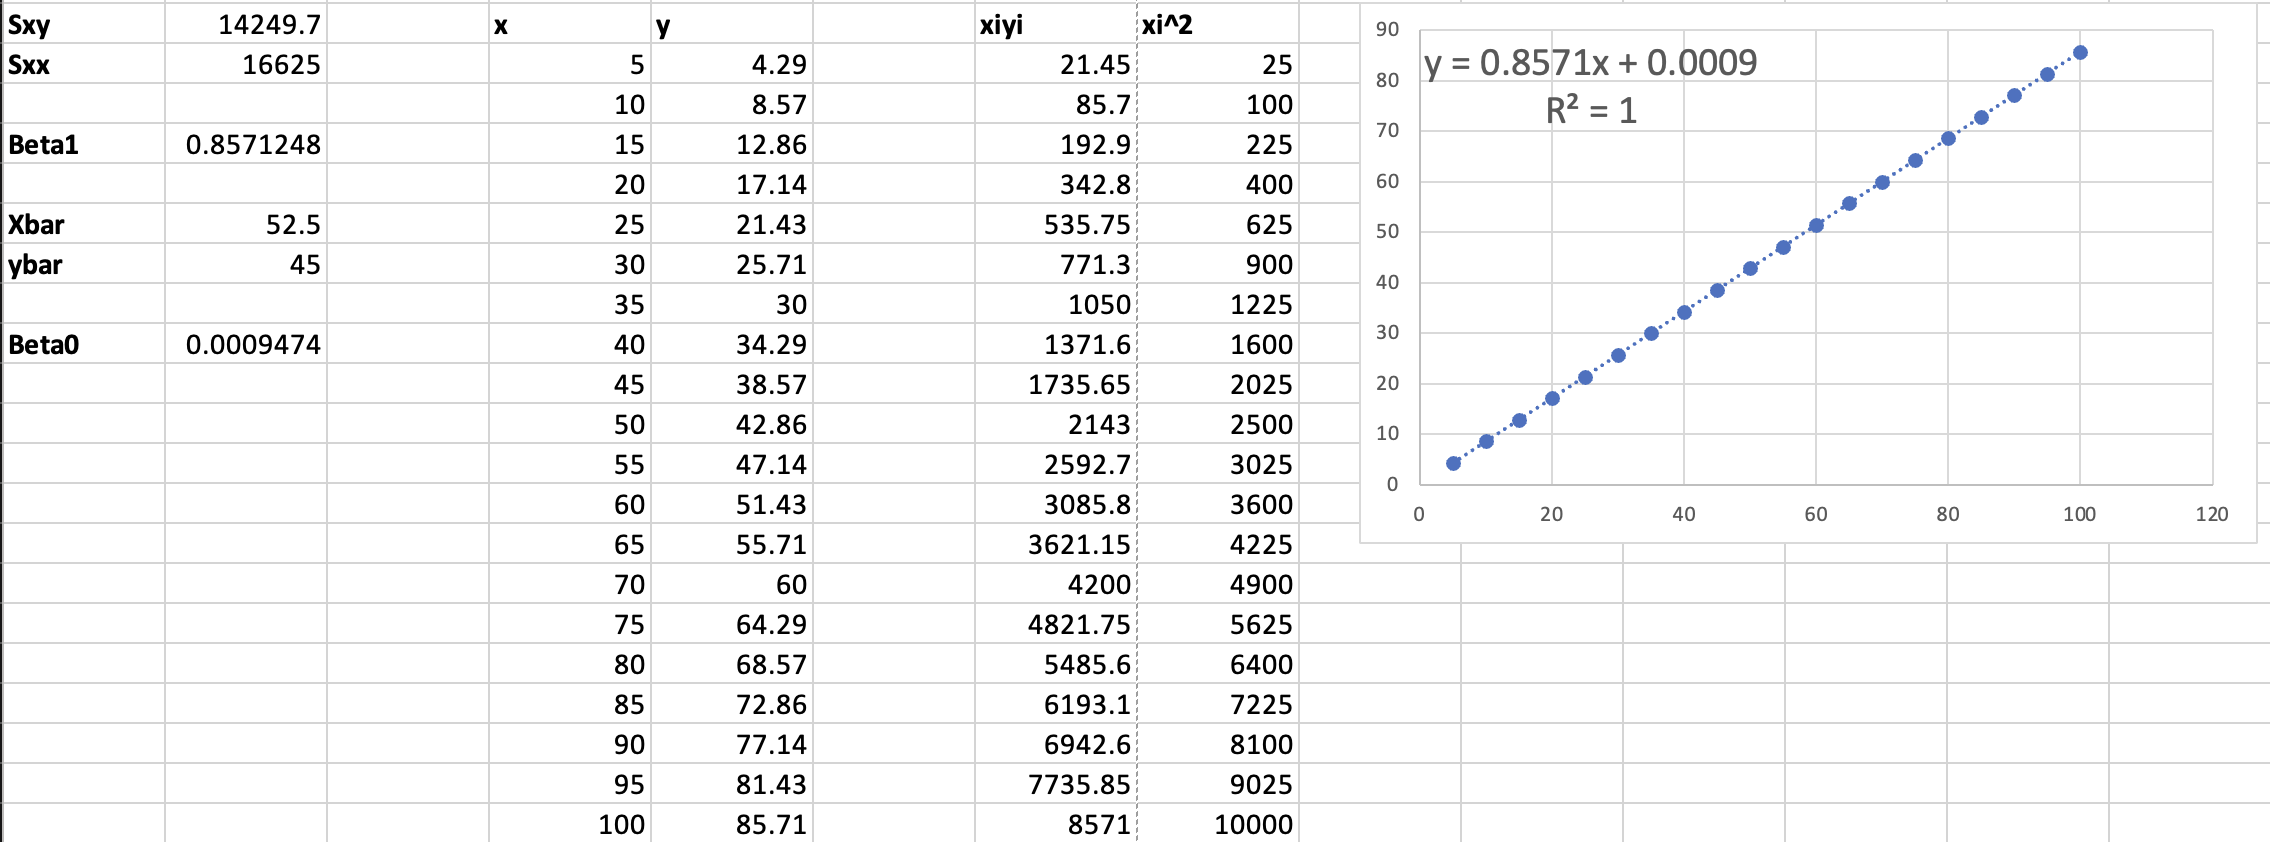
\includegraphics[scale=0.4]{./table.png}\]
Then,
\begin{enumerate}[label=(\alph*)]
\item \[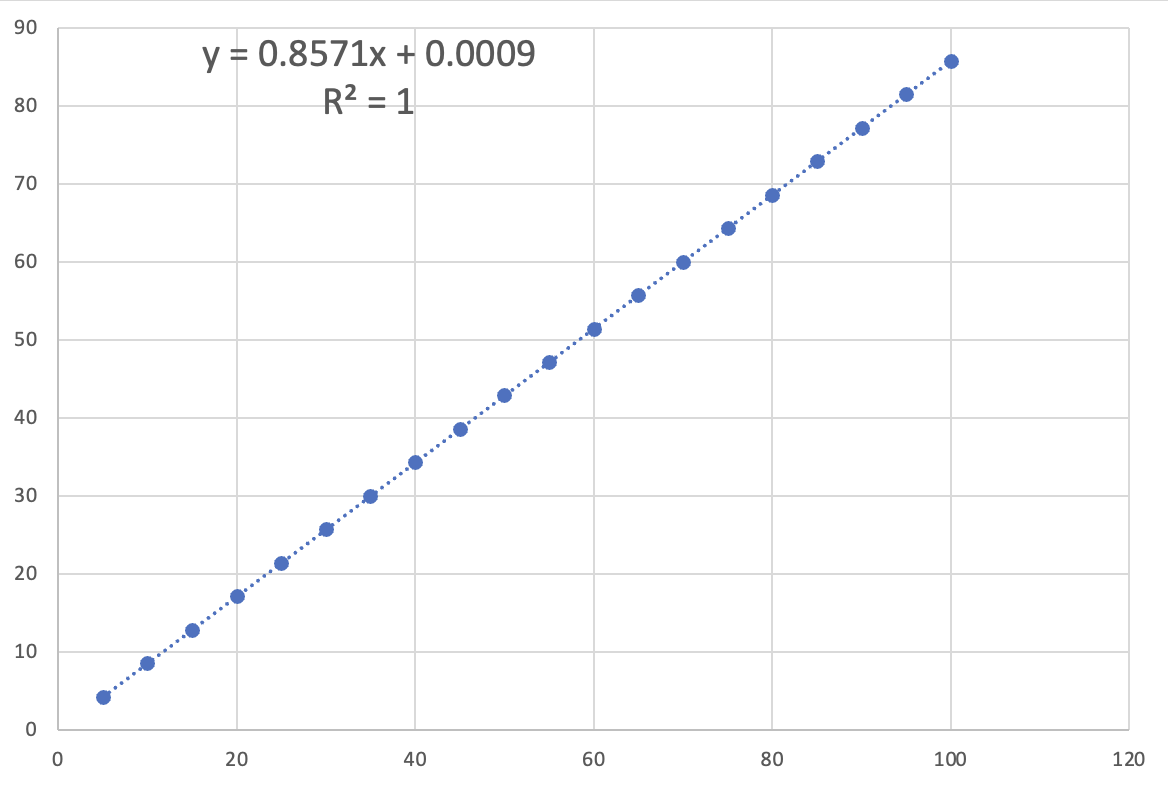
\includegraphics[scale=0.6]{./graph.png}\]
\item Given:
  \begin{align*}
    \hat{\beta_1} &= \frac{\sum\limits_{i = 1}^{N} (x_i - \overline{x})(y_i - \overline{y})}
                    {\sum\limits_{i = 1}^{N} (x_i - \overline{x})^2} \\
                  &= \frac{S_{xy}}{S_{xx}} \\
                  &= 0.8571
  \end{align*}
  and $\hat{\beta_0} = \overline{y} - \hat{\beta_1} \overline{x} = 0.8571$ from excel.
  So, we get $\hat{\beta_0} = 0.0009, \ \hat{\beta_1} = 0.8571$ . \\ \\
  $\beta_0$ is the deflection when a load of 0KN is applied to the beam. \\
  $\beta_1$ is the rate of change of the deflection when the load is increased on the beam.
\end{enumerate}


\newpage
\section*{Question 2}
\begin{proof}
  We want to show that $\hat{y} = \hat{\beta_0} + \hat{\beta_1} x$ always goes through the point
  $(\overline{x}, \overline{y})$. Given
  \begin{align*}
    \hat{y} &= \hat{\beta_0} + \hat{\beta_1} x \\
    \overline{y} &= \hat{\beta_0} + \hat{\beta_1} \overline{x}
                 &= \overline{y} - \hat{\beta_1} \overline{x} + \hat{\beta_1} \overline{x} && \text{by definition} \\
                 &= \overline{y} - \hat{\beta_1} (\overline{x} - \overline{x}) \\
    \overline{y} &= \overline{y}
  \end{align*}
  So, $\hat{y}$ always goes through the point $(\overline{x}, \overline{y})$.
\end{proof}

\newpage
\section*{Question 3}
\begin{proof}
  \begin{align*}
    E(\beta_1) &= E \left( \frac{\sum\limits_{i = 1}^{N} (x_i - \overline{x}) Y_i}
                 {S_{xx}} \right) \\
               &= \frac{\sum\limits_{i = 1}^{N} (x_i - \overline{x}) E(Y_i)}
                 {S_{xx}} \\
               &= \frac{\sum\limits_{i = 1}^{N} (x_i - \overline{x}) (\beta_0 + \beta_1 x_i)}{S_{xx}} \\
               &= \beta_0 \frac{\sum\limits_{i = 1}^{N} (x_i - \overline{x})}{S_{xx}}
                 + \beta_1 \frac{\sum\limits_{i = 1}^{N} (x_i - \overline{x}) x_i}{S_{xx}} \\
               &= 0 + \beta_1 \frac{S_{xx}}{S_{xx}} && \sum\limits_{i = 1}^{N} (x_i - \overline{x}) = 0 \\
    E(\beta_1) &= \beta_1 && (*)
  \end{align*}
  and
  \begin{align*}
    E(\hat{\beta_0}) &= E(\overline{Y}) - E(\hat{\beta_1}) \overline{x} \\
                     &= \beta_0 + \beta_1 \overline{x} && \text{from } (*) \\
    E(\hat{\beta_0}) &= \beta_0
  \end{align*}
  Therefore, $\hat{\beta_0}, \ \hat{\beta_1}$ represent unbiased estimators of $\beta_0, \ \beta_1$
\end{proof}
\end{document}

%%% Local Variables:
%%% mode: latex
%%% TeX-master: t
%%% End:
